\documentclass[border=5pt]{standalone}
\usepackage{tikz}
\usepackage{amsmath}
\usepackage{pgfplots}
\pgfplotsset{compat=1.18}
\begin{document}
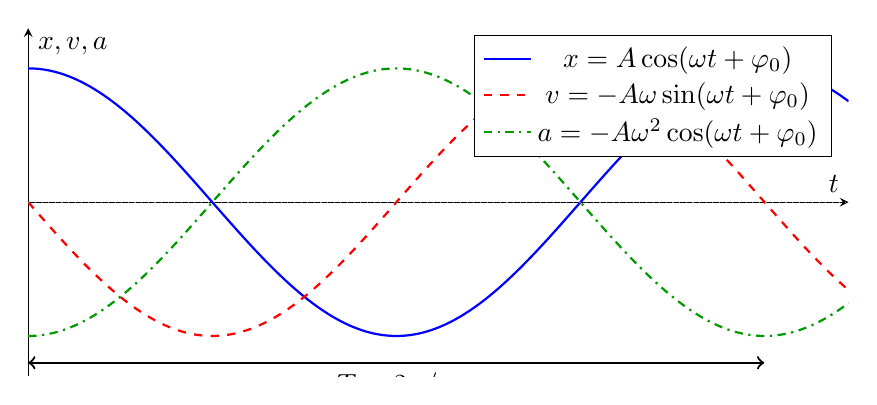
\begin{tikzpicture}
    \begin{axis}[
        width=12cm, height=6cm,
        xlabel={$t$},
        ylabel={$x, v, a$},
        xmin=0, xmax=7,
        ymin=-1.3, ymax=1.3,
        axis lines=middle,
        xtick=\empty,
        ytick=\empty,
        legend style={at={(0.98,0.98)}, anchor=north east},
        every axis plot/.append style={thick}
    ]
    % 位移 x = cos(t)
    \addplot[blue,domain=0:7,samples=200] {cos(deg(x))};
    \addlegendentry{$x = A\cos(\omega t + \varphi_0)$}
    
    % 速度 v = -sin(t)
    \addplot[red,dashed,domain=0:7,samples=200] {-sin(deg(x))};
    \addlegendentry{$v = -A\omega\sin(\omega t + \varphi_0)$}
    
    % 加速度 a = -cos(t)
    \addplot[green!60!black,dashdotted,domain=0:7,samples=200] {-cos(deg(x))};
    \addlegendentry{$a = -A\omega^2\cos(\omega t + \varphi_0)$}
    
    % 零点线
    \draw[gray,dotted] (axis cs:0,0) -- (axis cs:7,0);
    
    % 标注周期
    \draw[<->,thick] (axis cs:0,-1.2) -- (axis cs:6.28,-1.2);
    \node[below] at (axis cs:3.14,-1.2) {$T = 2\pi/\omega$};
    \end{axis}
\end{tikzpicture}
\end{document}
